\documentclass[final,1p,11pt]{elsarticle}

%\documentclass[final,1p,times]{elsarticle}


%% Use the option review to obtain double line spacing
%%\documentclass[authoryear,preprint,review,12pt]{elsarticle}

%% Use the options 1p,twocolumn; 3p; 3p,twocolumn; 5p; or 5p,twocolumn
%% for a journal layout:
%% \documentclass[final,1p,times]{elsarticle}
%% \documentclass[final,1p,times,twocolumn]{elsarticle}
%% \documentclass[final,3p,times]{elsarticle}
%% \documentclass[final,3p,times,twocolumn]{elsarticle}
%% \documentclass[final,5p,times]{elsarticle}
%% \documentclass[final,5p,times,twocolumn]{elsarticle}

%%% For including figures, graphicx.sty has been loaded in
%% elsarticle.cls. If you prefer to use the old commands
%% please give \usepackage{epsfig}


\usepackage{epsfig}
%\usepackage{cite}
%\usepackage{mcite}
\usepackage{array,tabularx,epsfig,mathrsfs,graphicx,rotating}
\usepackage{ifthen}
\usepackage{amsfonts}
\usepackage{ragged2e}
\PassOptionsToPackage{hyphens}{url}
\usepackage[hyphens]{url}
\usepackage{hyperref}
\usepackage{listings}
\usepackage{subfigure}
\usepackage{epstopdf}
% Custom colors
\usepackage{color}
\usepackage{float}
\usepackage{verbatim}

% to cross text
\usepackage[normalem]{ulem} % either use this (simple) or
\usepackage{soul} % use this (many fancier options)


\hypersetup{
  colorlinks=true,
  linkcolor=blue,
  citecolor=blue,
  urlcolor=blue
}




\graphicspath{{figs/}}


\pdfinfo{
   /Author (Chekanov et al)
   /Title  (Studies of granularity of a hadronic calorimeter for tens-of-TeV jets  at a 100 TeV pp collider)
   /CreationDate (D:2017)
   /Subject (PDFLaTeX)
   /Keywords (PDF;LaTeX)
}


\textheight=22cm
\textwidth=14.5cm

\newcommand{\beq}{\begin{equation}}
\newcommand{\eeq}{\end{equation}}
\newcommand{\la}{\langle}
\newcommand{\promc}{{\sc ProMC}}
\newcommand{\ra}{\rangle}
\newcommand{\eps}{\epsilon}
\newcommand{\ud}{\mathrm{d}}
\newcommand{\Ec}{\mathcal{E}}
\newcommand{\Fc}{\mathcal{F}}
\newcommand{\Za}{\mathrm{Z_1}}
\newcommand{\Zb}{\mathrm{Z_2}}
\newcommand{\Zn}{\mathrm{Z_n}}
\newcommand{\F}{\mathrm{F}}

\chardef\til=126
\newcommand{\mev}{{\,\mathrm{MeV}}}
\newcommand{\gev}{{\,\mathrm{GeV}}}
\newcommand{\tev}{{\,\mathrm{TeV}}}
\newcommand{\GEANTfour} {\textsc{geant4}}
\newcommand{\pythia} {\textsc{Pythia8}}


\journal{XXX-XXX}



\begin{document}
\section{Soft drop mass in future collider performance}
In this section, we use the specific method about the soft-drop to study the performance of the detector in the different detector cell sizes in different center-of-mass(c.m.) energy.  In the Figure , , , , are the distribution of the signal and background. 
\section{The theory of Soft drop}
Soft-drop, take literally, is the technique that can drop the soft mass which is smaller than set threshold. The formula is as following:
\begin{equation} \label{eq:soft-drop}
\frac{min(PT_{1},PT_{2})}{PT_{1}+PT_{2}}>Z_{cut}(\frac{\Delta R_{12}}{R_{0}}^{\beta})
\end{equation}
$PT_{1}$,$PT_{2}$ are the subjets when jets are declustered. $Z_{cut}$ is soft drop threshold. $\Delta R_{12}$ are the subjets distance in the rapidity-azimuth plane. $\beta$ is the exponent angular.
\begin{enumerate}
\item First, using the Anti-kt algorithm to reconstruct particles as many jets.
\item Second, starting our soft-drop task. Using the Cambridge-Aachen (C/A) algorithm to decluster the jets to the last step. Two subjets will emerge.
\item Third, comparing this two subjets in the formula \ref{eq:soft-drop}, if they pass, the original jets will be conserved. Nonetheless, removing the soft subjet, and using the bigger one to represent the original jet.
\item In the end, when the jets can't decluster to the subjets, it is done.
\end{enumerate}
By using a different $\beta$ value, the effect of selecting jets is different. In our study, we use $\beta=0$ and $\beta=2$. For $\beta=0$, the selection only depends on the $Z_{cut}$. For $\beta=2$, the selection depends on the angle of subjets and $Z_{cut}$, and it can remove both "soft" and "wid\subsection{Analysis method}
In this analysis, We fix the central at the median bin right boundary in signal distribution, and using the different width to draw ROC curves.
\subsection{The conclusion of the results}


 
%50bins
\begin{figure}
\begin{center}
   \subfigure[5TeV at 20$\times$20(cm$\times$cm) in cluster] {
   \includegraphics[width=0.22\textwidth]{figs/Dis_cluster_010_mass_mmdt_5tev_04.eps}
   }
      \subfigure[10TeV at 20$\times$20(cm$\times$cm) in cluster] {
   \includegraphics[width=0.22\textwidth]{figs/Dis_cluster_010_mass_mmdt_10tev_04.eps}
   }
   \subfigure[20TeV at 20$\times$20(cm$\times$cm) in cluster] {
   \includegraphics[width=0.22\textwidth]{figs/Dis_cluster_010_mass_mmdt_20tev_04.eps}
   }
    \subfigure[40TeV at 20$\times$20(cm$\times$cm) in cluster] {
   \includegraphics[width=0.22\textwidth]{figs/Dis_cluster_010_mass_mmdt_40tev_04.eps}
   }
   \subfigure[5TeV at 5$\times$5(cm$\times$cm) in cluster] {
   \includegraphics[width=0.22\textwidth]{figs/Dis_cluster_009_mass_mmdt_5tev_04.eps}
   }
   \subfigure[10TeV at 5$\times$5(cm$\times$cm) in cluster] {
   \includegraphics[width=0.22\textwidth]{figs/Dis_cluster_009_mass_mmdt_10tev_04.eps}
   }
      \subfigure[20TeV at 5$\times$5(cm$\times$cm) in cluster] {
   \includegraphics[width=0.22\textwidth]{figs/Dis_cluster_009_mass_mmdt_20tev_04.eps}\hfill
   }
      \subfigure[40TeV at 5$\times$5(cm$\times$cm) in cluster] {
   \includegraphics[width=0.22\textwidth]{figs/Dis_cluster_009_mass_mmdt_40tev_04.eps}\hfill
   }
   \subfigure[5TeV at 1$\times$1(cm$\times$cm) in cluster] {
   \includegraphics[width=0.22\textwidth]{figs/Dis_cluster_012_mass_mmdt_5tev_04.eps}\hfill
   }
    \subfigure[10TeV at 1$\times$1(cm$\times$cm) in cluster] {
   \includegraphics[width=0.22\textwidth]{figs/Dis_cluster_012_mass_mmdt_10tev_04.eps}
   }
   \subfigure[20TeV at 1$\times$1(cm$\times$cm) in cluster] {
   \includegraphics[width=0.22\textwidth]{figs/Dis_cluster_012_mass_mmdt_20tev_04.eps}\hfill
   }
      \subfigure[40TeV at 1$\times$1(cm$\times$cm) in cluster] {
   \includegraphics[width=0.22\textwidth]{figs/Dis_cluster_012_mass_mmdt_40tev_04.eps}
   }

\end{center}
\caption{Distributions of mass soft drop at $\beta$=0, signal=ww, in 5,10TeV energy of collision  in different detector sizes. Cell Size in 20$\times$20, 5$\times$5, and 1$\times$1(cm$\times$cm) are shown here.}
\label{fig:cluster_tau21_tau32}
\end{figure}

\begin{figure}
\begin{center}
  \subfigure[Central at Median($20\times20$=80,$5\times5$=80,$1\times1$=80) change width in cluster at 5TeV] {
  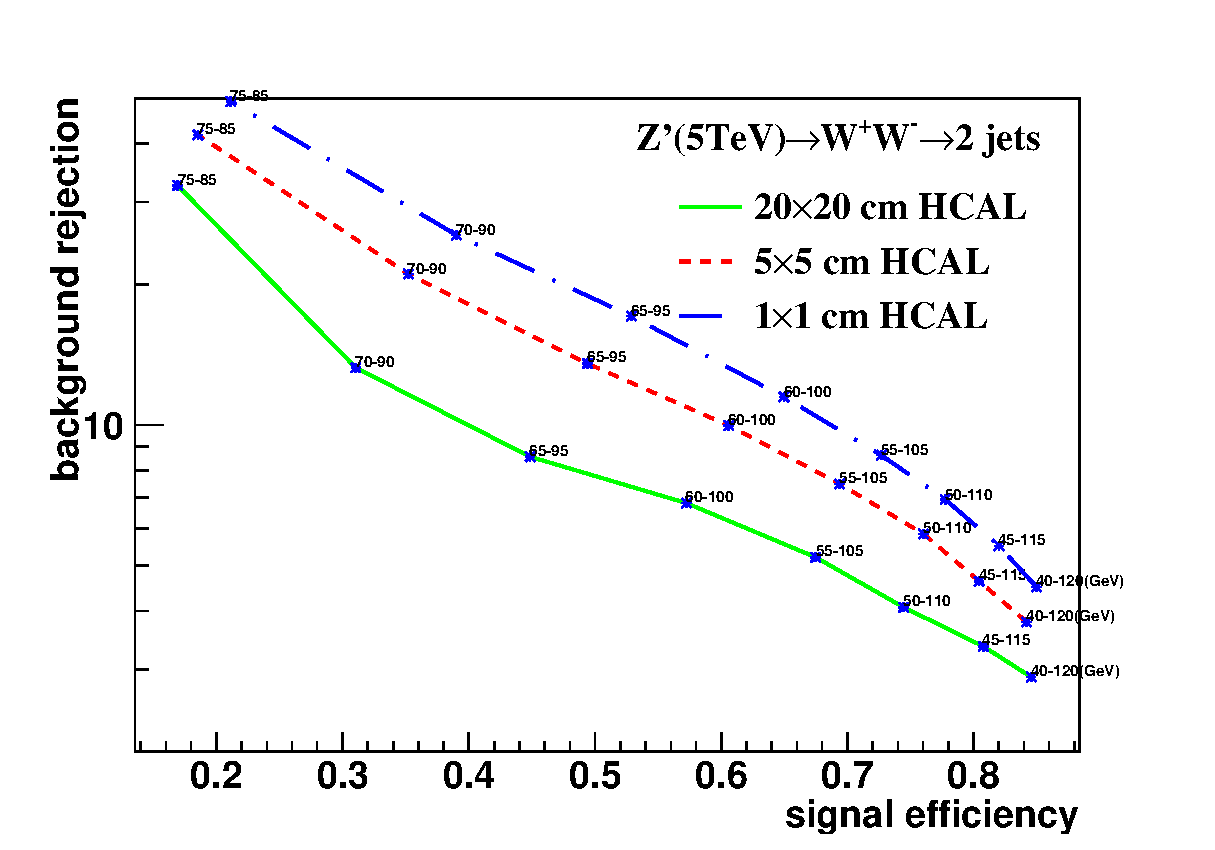
\includegraphics[width=0.43\textwidth]{figs/A_Cluster_mass_mmdt_5tev_eff_1_central_fix_ww_qq_log.eps}
  }
  \subfigure[Central at Median($20\times20$=95,$5\times5$=80,$1\times1$=75) change width in cluster at 10TeV] {
  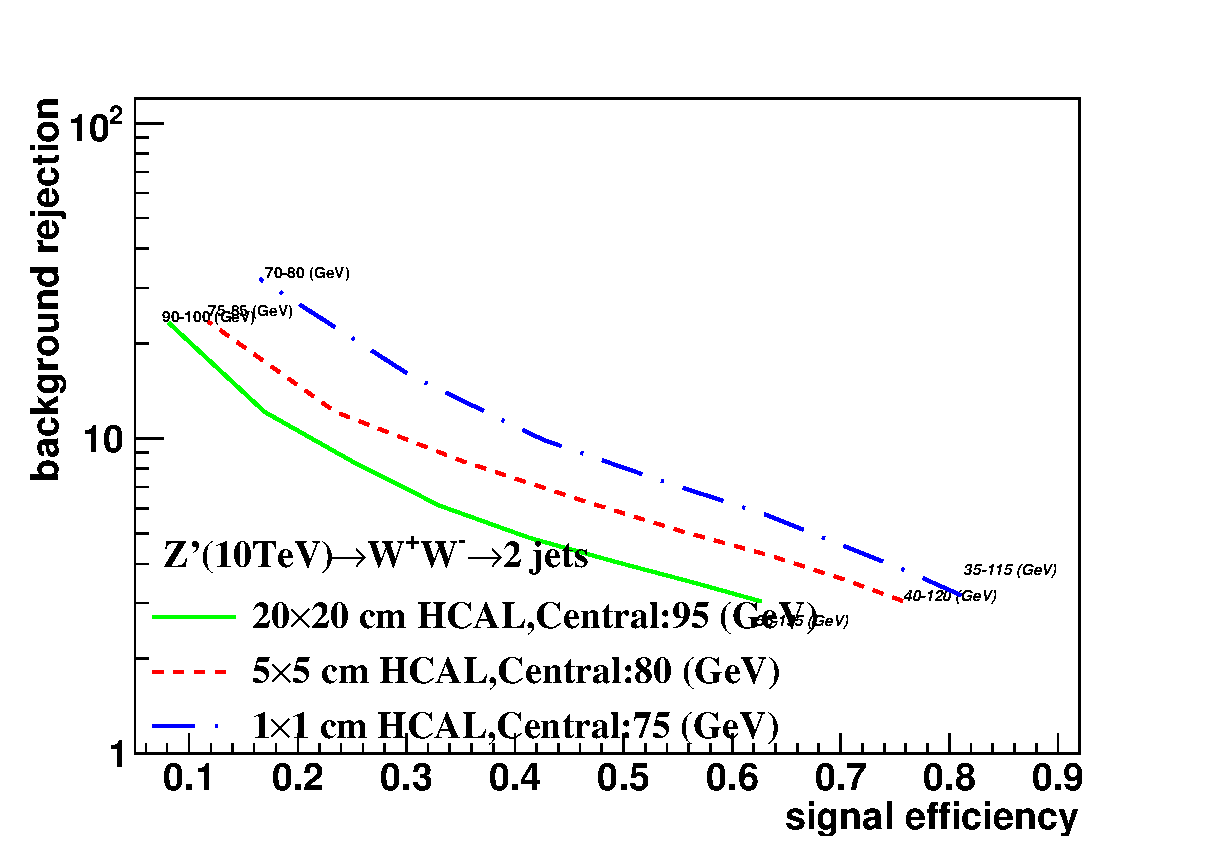
\includegraphics[width=0.43\textwidth]{figs/A_Cluster_mass_mmdt_10tev_eff_1_central_fix_ww_qq_log.eps}
  }
 \subfigure[Central at Median($20\times20$=155,$5\times5$=95,$1\times1$=90) change width in cluster at 20TeV] {
 \includegraphics[width=0.43\textwidth]{figs/A_Cluster_mass_mmdt_20tev_eff_1_central_fix_ww_qq_log.eps}
 }
 \subfigure[Central at Median($20\times20$=130,$5\times5$=150,$1\times1$=135) change width in cluster at 40TeV] {
 \includegraphics[width=0.43\textwidth]{figs/A_Cluster_mass_mmdt_40tev_eff_1_central_fix_ww_qq_log.eps}
 }
\end{center}
\caption{study of "fix central and change width" in mass soft drop at $\beta$=0, signal=ww, in 5, 10, 20, 40TeV energy of collision  in different detector sizes. Cell Size in 20$\times$20, 5$\times$5, and 1$\times$1(cm$\times$cm) are shown in each picture.}
\label{fig:cluster_tau21_tau32}
\end{figure}

\begin{figure}
\begin{center}
   \subfigure[5TeV at 20$\times$20(cm$\times$cm) in cluster] {
   \includegraphics[width=0.22\textwidth]{figs/Dis_cluster_010_mass_mmdt_tt_5tev_04_tt.eps}
   }
      \subfigure[10TeV at 20$\times$20(cm$\times$cm) in cluster] {
   \includegraphics[width=0.22\textwidth]{figs/Dis_cluster_010_mass_mmdt_tt_10tev_04_tt.eps}
   }
   \subfigure[20TeV at 5$\times$5(cm$\times$cm) in cluster] {
   \includegraphics[width=0.22\textwidth]{figs/Dis_cluster_010_mass_mmdt_tt_20tev_04_tt.eps}
   }
    \subfigure[40TeV at 5$\times$5(cm$\times$cm) in cluster] {
   \includegraphics[width=0.22\textwidth]{figs/Dis_cluster_010_mass_mmdt_tt_40tev_04_tt.eps}
   }
   \subfigure[5TeV at 1$\times$1(cm$\times$cm) in cluster] {
   \includegraphics[width=0.22\textwidth]{figs/Dis_cluster_009_mass_mmdt_tt_5tev_04_tt.eps}
   }
   \subfigure[10TeV at 1$\times$1(cm$\times$cm) in cluster] {
   \includegraphics[width=0.22\textwidth]{figs/Dis_cluster_009_mass_mmdt_tt_10tev_04_tt.eps}
   }
   \subfigure[20TeV at 20$\times$20(cm$\times$cm) in cluster] {
   \includegraphics[width=0.22\textwidth]{figs/Dis_cluster_009_mass_mmdt_tt_20tev_04_tt.eps}\hfill
   }
      \subfigure[40TeV at 20$\times$20(cm$\times$cm) in cluster] {
   \includegraphics[width=0.22\textwidth]{figs/Dis_cluster_009_mass_mmdt_tt_40tev_04_tt.eps}\hfill
   }
   \subfigure[5TeV at 5$\times$5(cm$\times$cm) in cluster] {
   \includegraphics[width=0.22\textwidth]{figs/Dis_cluster_012_mass_mmdt_tt_5tev_04_tt.eps}\hfill
   }
    \subfigure[10TeV at 5$\times$5(cm$\times$cm) in cluster] {
   \includegraphics[width=0.22\textwidth]{figs/Dis_cluster_012_mass_mmdt_tt_10tev_04_tt.eps}
   }
   \subfigure[20TeV at 1$\times$1(cm$\times$cm) in cluster] {
   \includegraphics[width=0.22\textwidth]{figs/Dis_cluster_012_mass_mmdt_tt_20tev_04_tt.eps}\hfill
   }
      \subfigure[40TeV at 1$\times$1(cm$\times$cm) in cluster] {
   \includegraphics[width=0.22\textwidth]{figs/Dis_cluster_012_mass_mmdt_tt_40tev_04_tt.eps}
   }
\end{center}
\caption{Distributions of mass soft drop at $\beta$=0, signal=tt, in 5,10TeV energy of collision  in different detector sizes. Cell Size in 20$\times$20, 5$\times$5, and 1$\times$1(cm$\times$cm) are shown here.}
\label{fig:cluster_tau21_tau32}
\end{figure}

\begin{figure}
\begin{center}
  \subfigure[Central at Median($20\times20$=150,$5\times5$=150,$1\times1$=150) change width in cluster at 5TeV] {
  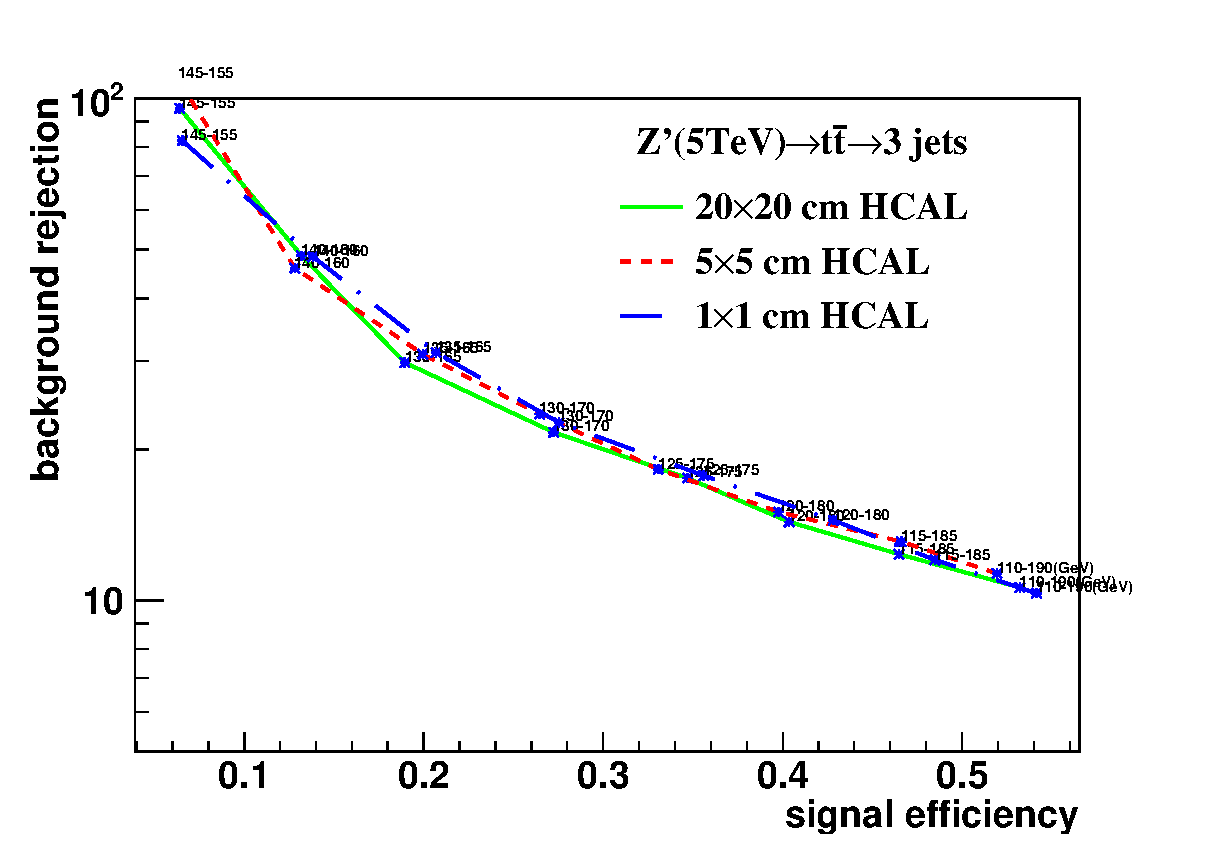
\includegraphics[width=0.43\textwidth]{figs/A_Cluster_mass_mmdt_5tev_eff_1_central_fix_tt_qq_log.eps}
  }
  \subfigure[Central at Median($20\times20$=155,$5\times5$=150,$1\times1$=155) change width in cluster at 10TeV] {
  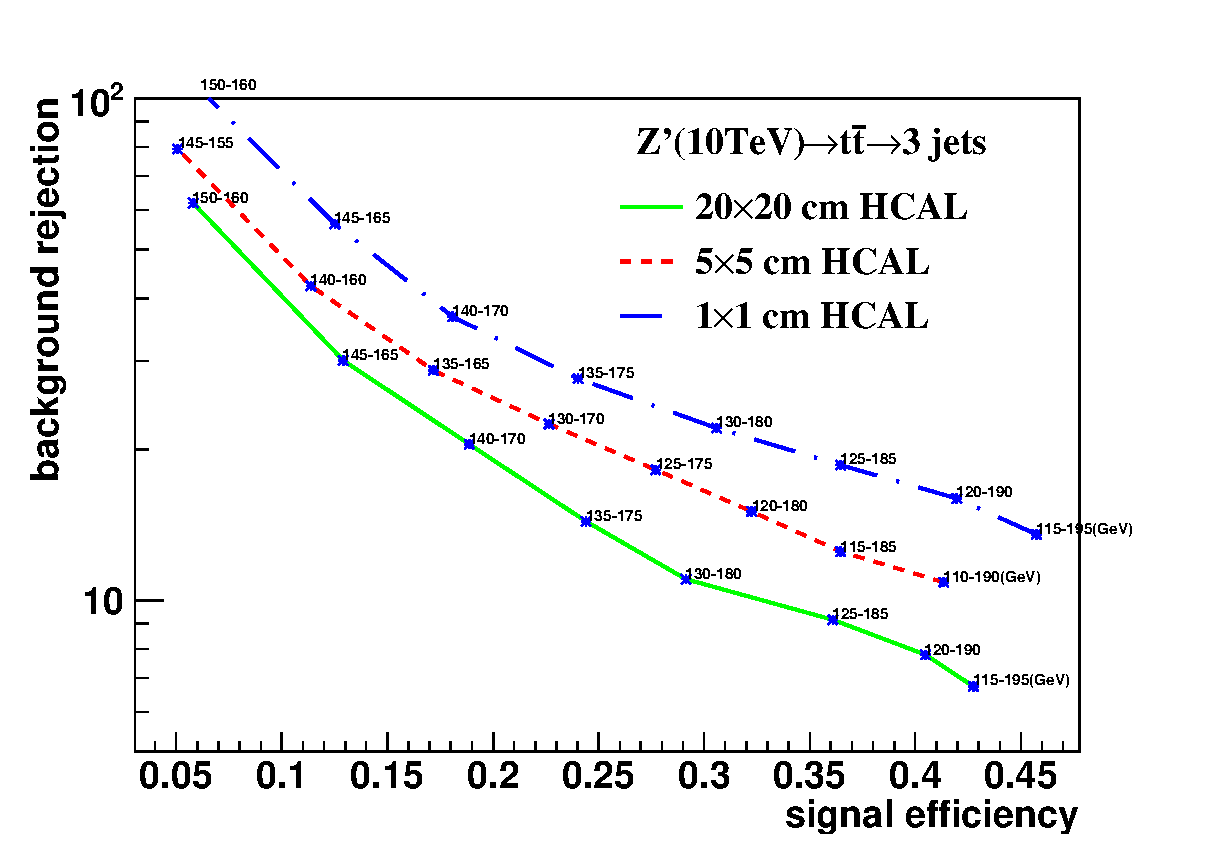
\includegraphics[width=0.43\textwidth]{figs/A_Cluster_mass_mmdt_10tev_eff_1_central_fix_tt_qq_log.eps}
  }
 \subfigure[Central at Median($20\times20$=165,$5\times5$=175,$1\times1$=170) change width in cluster at 20TeV] {
 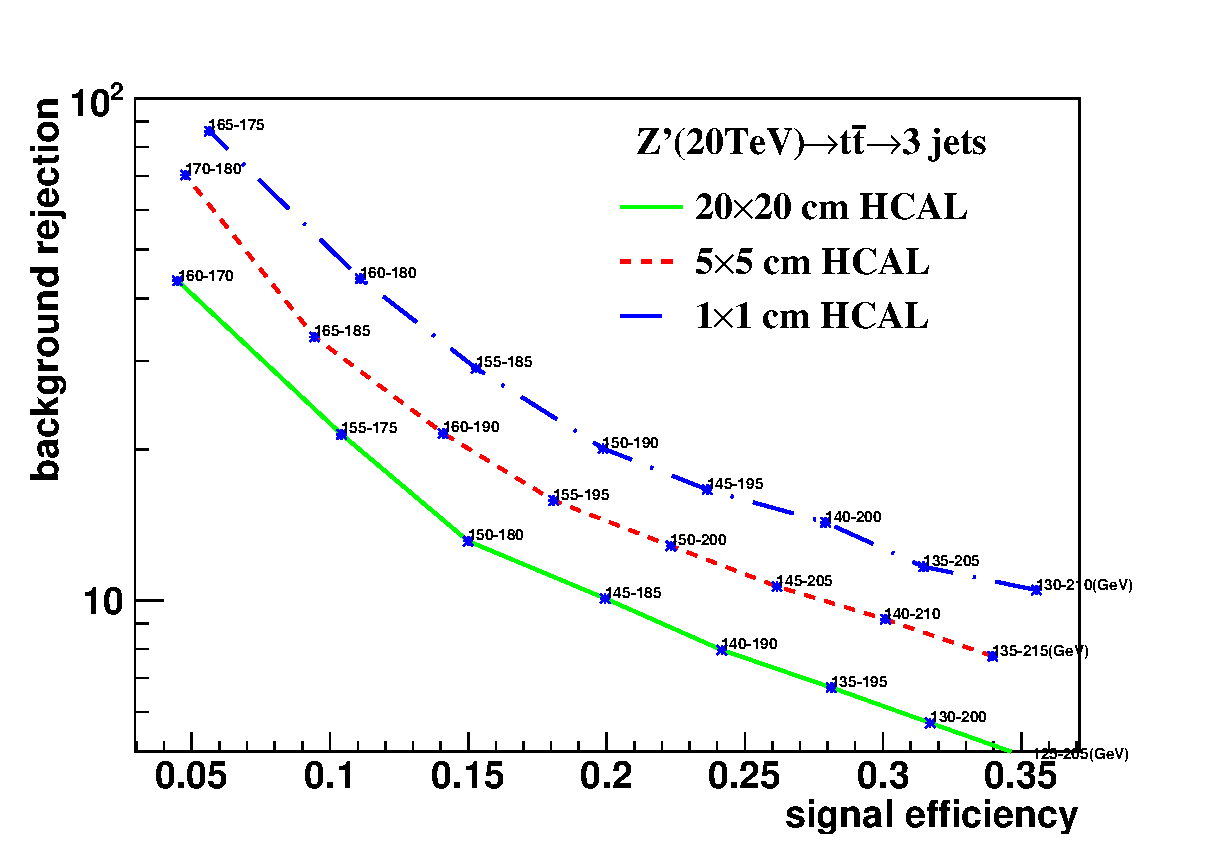
\includegraphics[width=0.43\textwidth]{figs/A_Cluster_mass_mmdt_20tev_eff_1_central_fix_tt_qq_log.eps}
 }
 \subfigure[Central at Median($20\times20$=190,$5\times5$=200,$1\times1$=190) change width in cluster at 40TeV] {
 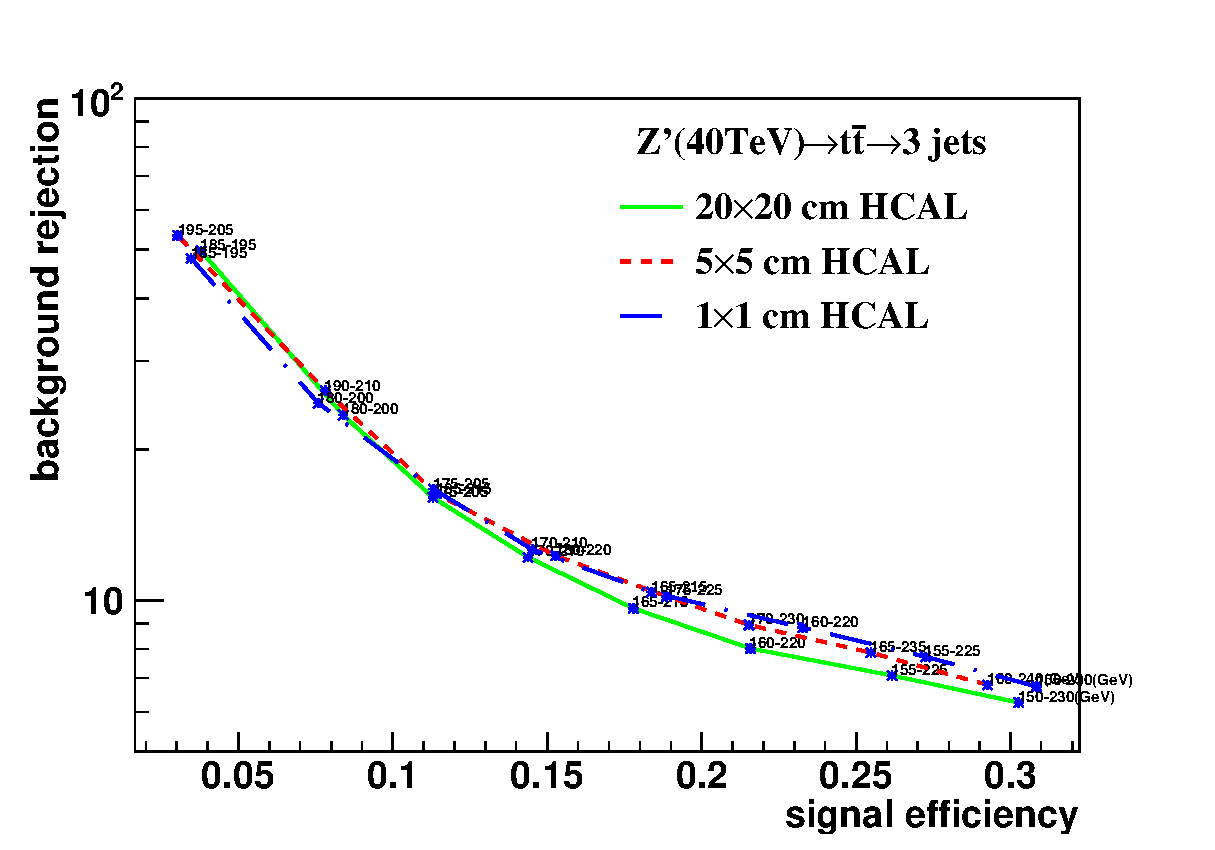
\includegraphics[width=0.43\textwidth]{figs/A_Cluster_mass_mmdt_40tev_eff_1_central_fix_tt_qq_log.eps}
 }
\end{center}
\caption{study of "fix central and change width" in mass soft drop at $\beta$=0, signal=tt, in 5, 10, 20, 40TeV energy of collision  in different detector sizes. Cell Size in 20$\times$20, 5$\times$5, and 1$\times$1(cm$\times$cm) are shown in each picture.}
\label{fig:cluster_tau21_tau32}
\end{figure}


\begin{figure}
\begin{center}
   \subfigure[5TeV at 20$\times$20(cm$\times$cm) in cluster] {
   \includegraphics[width=0.22\textwidth]{figs/Dis_cluster_010_mass_sdb2_ww_5tev_04_800.eps}
   }
      \subfigure[10TeV at 20$\times$20(cm$\times$cm) in cluster] {
   \includegraphics[width=0.22\textwidth]{figs/Dis_cluster_010_mass_sdb2_ww_10tev_04_800.eps}
   }
   \subfigure[20TeV at 20$\times$20(cm$\times$cm) in cluster] {
   \includegraphics[width=0.22\textwidth]{figs/Dis_cluster_010_mass_sdb2_ww_20tev_04_1600.eps}
   }
    \subfigure[40TeV at 20$\times$20(cm$\times$cm) in cluster] {
   \includegraphics[width=0.22\textwidth]{figs/Dis_cluster_010_mass_sdb2_ww_40tev_04_1600.eps}
   }
   \subfigure[5TeV at 5$\times$5(cm$\times$cm) in cluster] {
   \includegraphics[width=0.22\textwidth]{figs/Dis_cluster_009_mass_sdb2_ww_5tev_04_800.eps}
   }
   \subfigure[10TeV at 5$\times$5(cm$\times$cm) in cluster] {
   \includegraphics[width=0.22\textwidth]{figs/Dis_cluster_009_mass_sdb2_ww_10tev_04_800.eps}
   }
    \subfigure[20TeV at 5$\times$5(cm$\times$cm) in cluster] {
   \includegraphics[width=0.22\textwidth]{figs/Dis_cluster_009_mass_sdb2_ww_20tev_04_1600.eps}\hfill
   }
      \subfigure[40TeV at 5$\times$5(cm$\times$cm) in cluster] {
   \includegraphics[width=0.22\textwidth]{figs/Dis_cluster_009_mass_sdb2_ww_40tev_04_1600.eps}\hfill
   }
   \subfigure[5TeV at 1$\times$1(cm$\times$cm) in cluster] {
   \includegraphics[width=0.22\textwidth]{figs/Dis_cluster_012_mass_sdb2_ww_5tev_04_800.eps}\hfill
   }
    \subfigure[10TeV at 1$\times$1(cm$\times$cm) in cluster] {
   \includegraphics[width=0.22\textwidth]{figs/Dis_cluster_012_mass_sdb2_ww_10tev_04_800.eps}
   }
   \subfigure[20TeV at 1$\times$1(cm$\times$cm) in cluster] {
   \includegraphics[width=0.22\textwidth]{figs/Dis_cluster_012_mass_sdb2_ww_20tev_04_1600.eps}\hfill
   }
      \subfigure[40TeV at 1$\times$1(cm$\times$cm) in cluster] {
   \includegraphics[width=0.22\textwidth]{figs/Dis_cluster_012_mass_sdb2_ww_40tev_04_1600.eps}
   }
\end{center}
\caption{Distributions of mass soft drop at $\beta$=2, signal=ww, in 5,10TeV energy of collision  in different detector sizes. Cell Size in 20$\times$20, 5$\times$5, and 1$\times$1(cm$\times$cm) are shown here.}
\label{fig:cluster_tau21_tau32}
\end{figure}


\begin{figure}
\begin{center}
  \subfigure[Central at Median($20\times20$=115,$5\times5$=110,$1\times1$=115) change width in cluster at 5TeV] {
  \includegraphics[width=0.43\textwidth]{figs/A_Cluster_mass_sdb2_5tev_eff_1_central_fix_ww_qq_log.eps}
  }
  \subfigure[Central at Median($20\times20$=155,$5\times5$=140,$1\times1$=145) change width in cluster at 10TeV] {
  \includegraphics[width=0.43\textwidth]{figs/A_Cluster_mass_sdb2_10tev_eff_1_central_fix_ww_qq_log.eps}
  }
 \subfigure[Central at Median($20\times20$=250,$5\times5$=195,$1\times1$=205) change width in cluster at 20TeV] {
 \includegraphics[width=0.43\textwidth]{figs/A_Cluster_mass_sdb2_20tev_eff_1_central_fix_ww_qq_log.eps}
 }
 \subfigure[Central at Median($20\times20$=285,$5\times5$=310,$1\times1$=290) change width in cluster at 40TeV] {
 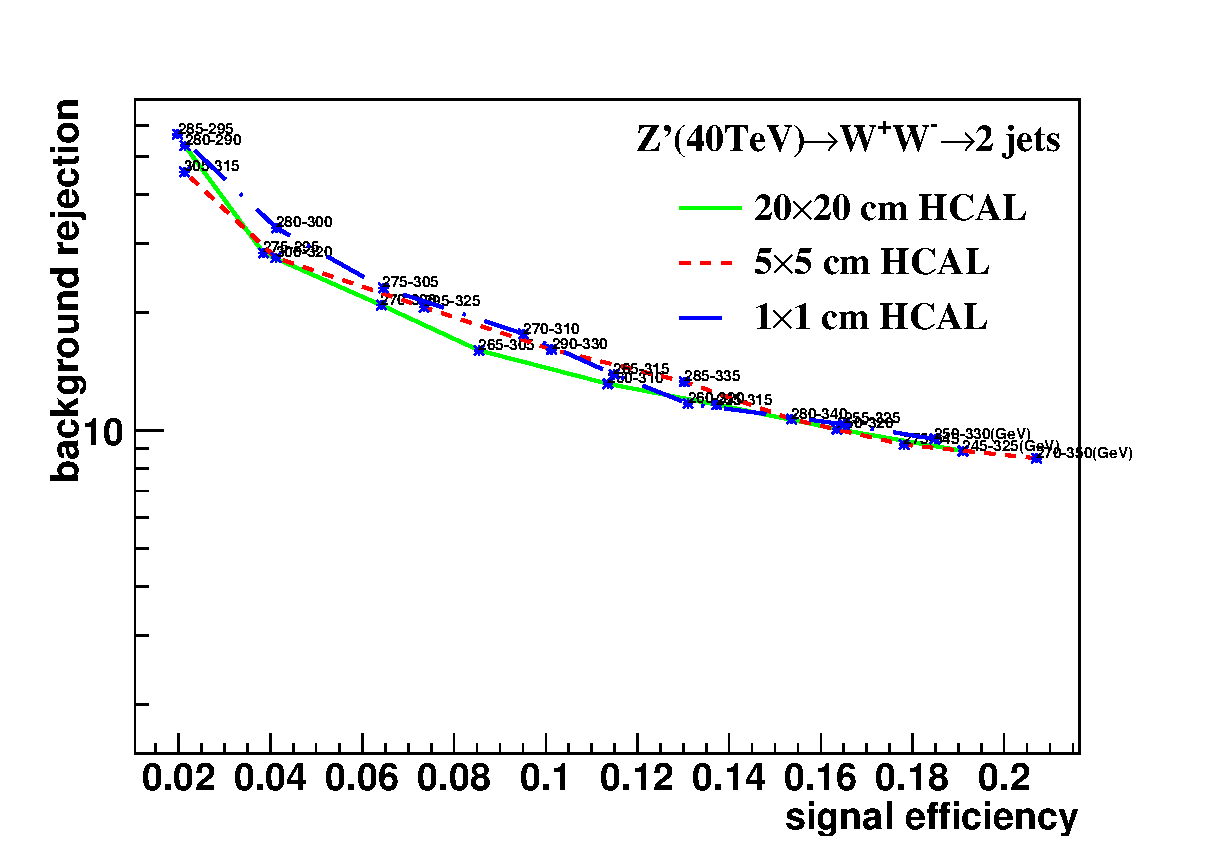
\includegraphics[width=0.43\textwidth]{figs/A_Cluster_mass_sdb2_40tev_eff_1_central_fix_ww_qq_log.eps}
 }
\end{center}
\caption{study of "fix central and change width" in mass soft drop at $\beta$=2, signal=ww, in 5, 10, 20, 40TeV energy of collision  in different detector sizes. Cell Size in 20$\times$20, 5$\times$5, and 1$\times$1(cm$\times$cm) are shown in each picture.}
\label{fig:cluster_tau21_tau32}
\end{figure}

\begin{figure}
\begin{center}
   \subfigure[5TeV at 20$\times$20(cm$\times$cm) in cluster] {
   \includegraphics[width=0.22\textwidth]{figs/Dis_cluster_012_mass_sdb2_tt_5tev_04_tt_1200.eps}
   }
      \subfigure[10TeV at 20$\times$20(cm$\times$cm) in cluster] {
   \includegraphics[width=0.22\textwidth]{figs/Dis_cluster_010_mass_sdb2_tt_10tev_04_tt_1200.eps}
   }
   \subfigure[20TeV at 20$\times$20(cm$\times$cm) in cluster] {
   \includegraphics[width=0.22\textwidth]{figs/Dis_cluster_010_mass_sdb2_tt_20tev_04_tt_2400.eps}
   }
    \subfigure[40TeV at 20$\times$20(cm$\times$cm) in cluster] {
   \includegraphics[width=0.22\textwidth]{figs/Dis_cluster_010_mass_sdb2_tt_40tev_04_tt_2400.eps}
   }
   \subfigure[5TeV at 5$\times$5(cm$\times$cm) in cluster] {
   \includegraphics[width=0.22\textwidth]{figs/Dis_cluster_009_mass_sdb2_tt_5tev_04_tt_1200.eps}
   }
   \subfigure[10TeV at 5$\times$5(cm$\times$cm) in cluster] {
   \includegraphics[width=0.22\textwidth]{figs/Dis_cluster_009_mass_sdb2_tt_10tev_04_tt_1200.eps}
   }
   \subfigure[20TeV at 5$\times$5(cm$\times$cm) in cluster] {
   \includegraphics[width=0.22\textwidth]{figs/Dis_cluster_009_mass_sdb2_tt_20tev_04_tt_2400.eps}\hfill
   }
      \subfigure[40TeV at 5$\times$5(cm$\times$cm) in cluster] {
   \includegraphics[width=0.22\textwidth]{figs/Dis_cluster_009_mass_sdb2_tt_40tev_04_tt_2400.eps}\hfill
   }
   \subfigure[5TeV at 1$\times$1(cm$\times$cm) in cluster] {
   \includegraphics[width=0.22\textwidth]{figs/Dis_cluster_012_mass_sdb2_tt_5tev_04_tt_1200.eps}\hfill
   }
    \subfigure[10TeV at 1$\times$1(cm$\times$cm) in cluster] {
   \includegraphics[width=0.22\textwidth]{figs/Dis_cluster_012_mass_sdb2_tt_10tev_04_tt_1200.eps}
   }
   \subfigure[20TeV at 1$\times$1(cm$\times$cm) in cluster] {
   \includegraphics[width=0.22\textwidth]{figs/Dis_cluster_012_mass_sdb2_tt_20tev_04_tt_2400.eps}\hfill
   }
      \subfigure[40TeV at 1$\times$1(cm$\times$cm) in cluster] {
   \includegraphics[width=0.22\textwidth]{figs/Dis_cluster_012_mass_sdb2_tt_40tev_04_tt_2400.eps}
   }
\end{center}
\caption{Distributions of mass soft drop at $\beta$=2, signal=tt, in 5,10TeV energy of collision  in different detector sizes. Cell Size in 20$\times$20, 5$\times$5, and 1$\times$1(cm$\times$cm) are shown here.}
\label{fig:cluster_tau21_tau32}
\end{figure}


\begin{figure}
\begin{center}
  \subfigure[Central at Median($20\times20$=185,$5\times5$=185,$1\times1$=185) change width in cluster at 5TeV] {
  \includegraphics[width=0.43\textwidth]{figs/A_Cluster_mass_sdb2_5tev_eff_1_central_fix_tt_qq_log.eps}
  }
  \subfigure[Central at Median($20\times20$=240,$5\times5$=240,$1\times1$=240) change width in cluster at 10TeV] {
  \includegraphics[width=0.43\textwidth]{figs/A_Cluster_mass_sdb2_10tev_eff_1_central_fix_tt_qq_log.eps}
  }
 \subfigure[Central at Median($20\times20$=360,$5\times5$=375,$1\times1$=365) change width in cluster at 20TeV] {
 \includegraphics[width=0.43\textwidth]{figs/A_Cluster_mass_sdb2_20tev_eff_1_central_fix_tt_qq_log.eps}
 }
 \subfigure[Central at Median($20\times20$=620,$5\times5$=625,$1\times1$=630) change width in cluster at 40TeV] {
 \includegraphics[width=0.43\textwidth]{figs/A_Cluster_mass_sdb2_40tev_eff_1_central_fix_tt_qq_log.eps}
 }
\end{center}
\caption{study of "fix central and change width" in mass soft drop at $\beta$=2, signal=tt, in 5, 10, 20, 40TeV energy of collision  in different detector sizes. Cell Size in 20$\times$20, 5$\times$5, and 1$\times$1(cm$\times$cm) are shown in each picture.}
\label{fig:cluster_tau21_tau32}
\end{figure}

\end{document}



